\chapter{Power Management}
``It will also be interesting to look at Sapphire Rapids, which also implements Golden Cove cores, including an analysis of user space idle states, and AVX frequencies.''
\todoms{cite alder lake paper}
\todoms{what is in the outlook of the sklylake, cascade lake and icelake papers?}


\begin{itemize}
    \item highlight why throttling mechanisms exist.\\
    Iccmax. first droop. maybe cite patent and/or look in the source code of edk2.
    \item question: what uses power on the processor? (execution and memory movement)
\end{itemize}


\section{Infuence of Tiles}
\begin{itemize}
    \item one pmu per tile. one master pmu.\todoms{citations of the patent}
    \item find the location of the pmu. one measurement.\todoms{Where is the PMU?}
\end{itemize}

\section{Shared Frequency Domains}
% measurements/shared-frequency-domains 
Starting with Sapphire Rapids, Intel changed their design on server processors to have shared FIVR for a set of up to four cores~\cite{Intel_2022_ISSCC}.
This change requires us to validate that core frequencies are independent of each other.
We adopt the measurement scripts from Sch\"one et al~\cite{Schoene_2024_Alder_Lake}.

For the measurement we disabled C-states, changed the cores to the lowest frequency (\SI{800}{\MHz}) and run a while true loop on one core.
The frequency of this core has been measured while another core running at the highest frequency (\SI{3800}{\MHz}), either idling or also running a while true loop.
The measurement has been repeated for all combinations of cores on a socket.
We could not detect a change in frequency, therefore Sapphire Rapids must implements some scheme of frequency duty cycling for cores running with mixed frequencies on the same voltage regulator or let a core with a lower frequency core run with a suboptimal energy efficiency by using a higher than required voltage.
\todoms{Both options are not optimal, but the second should be worse in terms of EE.}

\section{AVX Frequencies}
\label{sec:avx-frequencies}

Starting with the Haswell Microarchitecture, Intel introduced the concept of AVX frequencies.
This allows AVX2 instructions to use a lower base and different per core turbo frequencies~\cite{Hackenberg_2015_Haswell}.
The concept has been extended with a new class for AVX512 instructions with the Skylake Server Microarchitecture~\cite[Sec. 2.6.3]{Intel_Optimization_Reference_Manual_050}.
With the introduction of Ice Lake these classes are not only determined by the instruction set or register size, but a more realistic model of actual power consumption by also classifing instruction into ``Light'' and ``Heavy'' classes by their power consumption~\cite{papazian_new_2020}.
With the addition of the AMX instruction set Intel split up these classes further ranging from ``Ultra-Light'' to ``Heavy''.
The used instruction set together with the power consumption are mapped to four license levels which determine the opportunistic AVX turbo frequencies based on the number of active cores.
The mapping from instruction set and power usage are displayed in~\tabref{avx-classes}~\cite{ServeTheHome_Emerald_Rapids_2023}.
In \figref{p0n-frequencies} we are able to extracte the per core opportunistic turbo frequencies per license on our testsystem using a modified version of ``intel-speed-select''.
\todoms{Reference to the test system}

% \begin{table}[t]
% 	\centering
% 	\caption{\label{tab:avx-classes}AVX frequency classes based on published slides from Intel.~\cite{ServeTheHome_Emerald_Rapids_2023}}
% 	\begin{tabular}{|l|c|c|c|c|}
%         \hline
%         \diagbox[height=5em]{Instruction\\Class}{\\$C_{dyn}$ Class} & 0 & 1 & 2 & 3 \\
%         \hline
%         SSE & 128 Light & 128 Heavy & & \\
%         AVX2 & 256 Light & 256 Moderate & 256 Heavy & \\
%         AVX512 & 512 Ultra-Light & 512 Light & 512 Moderate & 512 Heavy \\
%         AMX & & AMX Light & AMX Moderate & AMX Heavy \\
%         \hline \hline
%         Turbo Frequency & SSE & AVX2 & AVX512 & AMX \\ 
%         \hline
% 	\end{tabular}
% \end{table}

\begin{table}[t]
	\centering
	\caption{\label{tab:avx-classes}AVX frequency classes based on published slides from Intel.
    The $C_{dyn}$ classes 0 through 3 map to the license levels SSE, AVX2, AVX512 and AMX~\cite{ServeTheHome_Emerald_Rapids_2023}.
    The license levels that we could measure are marked in red.}
    \begin{tabular}{|l|p{0.14\textwidth}|p{0.17\textwidth}|p{0.17\textwidth}|p{0.17\textwidth}|}
        \hline
        \diagbox[width=0.24\textwidth]{$C_{dyn}$\\Class}{Instruction\\Class} & SSE & AVX2 & AVX512 & AMX \\
        \hline
        0 (SSE Frequency) & 128 Light & \cellcolor{red!15}{\textbf{256 Light}} & 512 Ultra-Light & \\
        \hline
        1 (AVX2 Frequency) & 128 Heavy & \cellcolor{red!15}{\textbf{256 Moderate}} & 512 Light & AMX Light \\
        \hline
        2 (AVX512 Frequency) & & 256 Heavy & \cellcolor{red!15}{\textbf{512 Moderate}} & AMX Moderate \\
        \hline
        3 (AMX Frequency) & & & \cellcolor{red!15}{\textbf{512 Heavy}} & AMX Heavy \\
        \hline
	\end{tabular}
\end{table}

In~\cite{Downs_2020_AVX_Downclocking}, Downs measured the influence of AVX throttling on Ice Lake by infering the license level based on the resulting frequency of the ``avx-turbo'' microarchitectural benchmark.
However they were only able to trigger two out of the three license level, leaving open the question on how instructions are mapped to ``Light'' and ``Heavy'' classes.
Laukemann et al.~\cite{laukemann_microarchitectural_2024} showed the same for Sapphire Rapids using ``likwid-bench'' with the ``peakflops\_avx512\_fma'' and ``peakflops\_avx\_fma'' microarchitectural benchmark.
They we also only able to show two out of the four license levels.

\begin{figure}[]
    \centering
    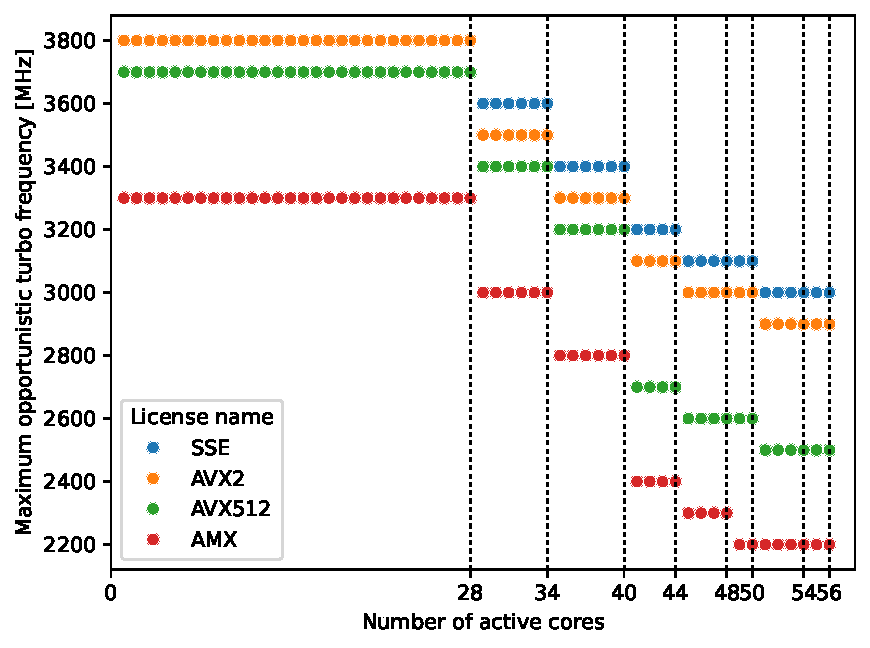
\includegraphics[width=0.8\columnwidth]{fig/avx-frequency-license-bands.pdf}
    \caption{\label{fig:p0n-frequencies}Opportunistic AVX turbo frequencies of the test system extracted using Intel Speed Select Technology.
    The number of active cores are split into eight buckets. The license and the bucket decides the resulting turbo frequency.
    In the first bucket the SSE and AVX2 license bands share the same frequency.}
\end{figure}

Register Address: 1ADH, 429 MSR\_TURBO\_RATIO\_LIMIT
Register Address: 1AEH, 430 MSR\_TURBO\_RATIO\_LIMIT\_CORES

\todoms{Show the license levels on SPR barnard (same processor as laukemann)}

\todoms{explain cdyn bench measurement}

% We propose a method to measure if small kernels trigger the power management of a core to stay in one license level.
To associate which events trigger the processor cores to be part of a license level, we design a microbenchmark that executes small kernels on a fixed number of threads and measure the resulting core frequencies.
This methodology is fundamentaly the same as demostrated by Downs and Laukemann et al.
However, we can only read the license level based on the maximal turbo frequency.
To ensure that we do not trigger other power limiting mechanisms, e.g. RAPL, we utilize ``Intel Speed Select Core-Power'' to set one thread to priority group zero and all other to priority group 1 with a fixed low maximum frequency.
The measurement of frequency is done on the thread in group zero, which should run at the maximum turbo frequency.
We will dissect ``Intel Speed Select'' in~\secref{isst}.

To validate the claim that the frequency limiting is independent of the ``Intel Speed Select Core-Power'' mechanisms, we prototype this measurement with four different FIRESTARTER kernels.
The result is displayed in~\figref{validated-p0n-frequencies}. We can clearly validate the findings of~\figref{p0n-frequencies}.
However, the power consumption of the AMX kernel has inconsistent jumps that change with multiple measurements.

\todoms{Display the different FIRESTARTER kernels and show that not only the user instruction set, but also the number of memory accesses are influencing the resulting license level.}

\todoms{Validate this claim: We have validated that a logic is triggering, different C state levels of unused threads or a change in uncore frequency?}


\begin{figure}[]
    \centering
    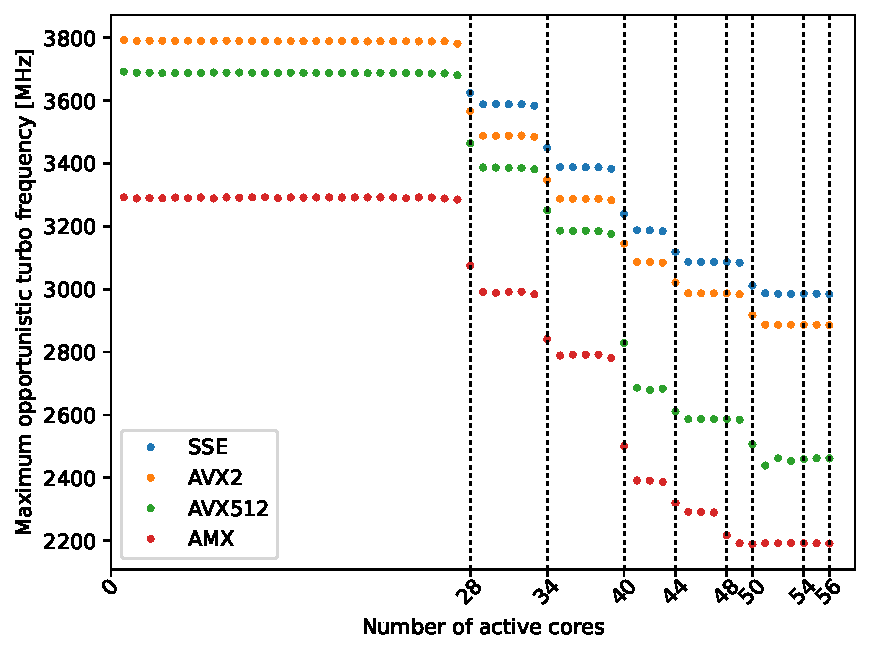
\includegraphics[width=0.8\columnwidth]{fig/validate-avx-frequency-license-bands.pdf}
    \caption{\label{fig:validated-p0n-frequencies}Validation of the opportunistic AVX turbo frequencies of the test system extracted using Intel Speed Select Technology.
    The number of active cores are split into eight buckets. The license and the bucket decides the resulting turbo frequency.
    In the first bucket the SSE and AVX2 license bands share the same frequency. We make shure that the package power does not exceed the maximum of \SI{350}{\watt} of our test platfrom.}
\end{figure}

\todoms{Rerun the measurements on banard.}

% \todoms{One plot with four Firestarter kernels, RAPL package vs max RAPL package on pkg0 with ISST, and frequency of thread zero to show that these two mechanisms are independent of each other. On all number of cores.}

\todoms{More details for cdyn measurement}


\begin{itemize}
    % \item one kernel on all cores of a socket -> we can read the frequency of the cores -> license.
    % \item problem: other throttling mechanisms (rapl).
    % intel speed select CLOS groups, one priority core, all other no priority.
    % we can read the frequency on the priority core.
    \item (again) question: what uses power on the processor? (execution and memory movement)
    why did the other two author fail at showing all levels?
    % \item Plot shows that memory accesses are important for changing the license level.
    \item make the case for memory size in loop and number of different instructions
    \item explain the kernels and their parameter.
    \item derive the rules for the classes
\end{itemize}

\todoms{How can we read the cdynn classes from the PMU (per core)?}
\todoms{How are instructions and memory accesses mapped to the cdynn classes?}

\section{Shared Voltage Domains}

Starting with Sapphire Rappids, Intel changed their design to have one one-die voltage regulator for multiple cores.
They are ''arranged in horizontal strips``~\cite{Intel_2022_ISSCC}.
This is a major change to their predecessors, where each core had its own FIVR.
\todoms{citation needed}
To measure this change, we run the same four FIRESTARTER workloads as described in~\secref{avx-frequencies}.
We repeat the measurement for different settings of the core, uncore frequency and different population order.
\todoms{describe the population order}

\todoms{how many (max four) and what cores (in rows) are on the same voltage regulator? We can detect 16 distinct jumps in power consumption when scaling a workload from one to all cores.}
\todoms{Plot power consumption for a stream workload running in L1 or L2, scaling the workload either over the rows or over the columns. We should get a plot with 16 distinct jumps spaced out and a plot with 16 jumps at the start and then a gradual increse.}
\todoms{shell script for mapping cpus to physical locations}

\begin{figure}[]
    \centering
    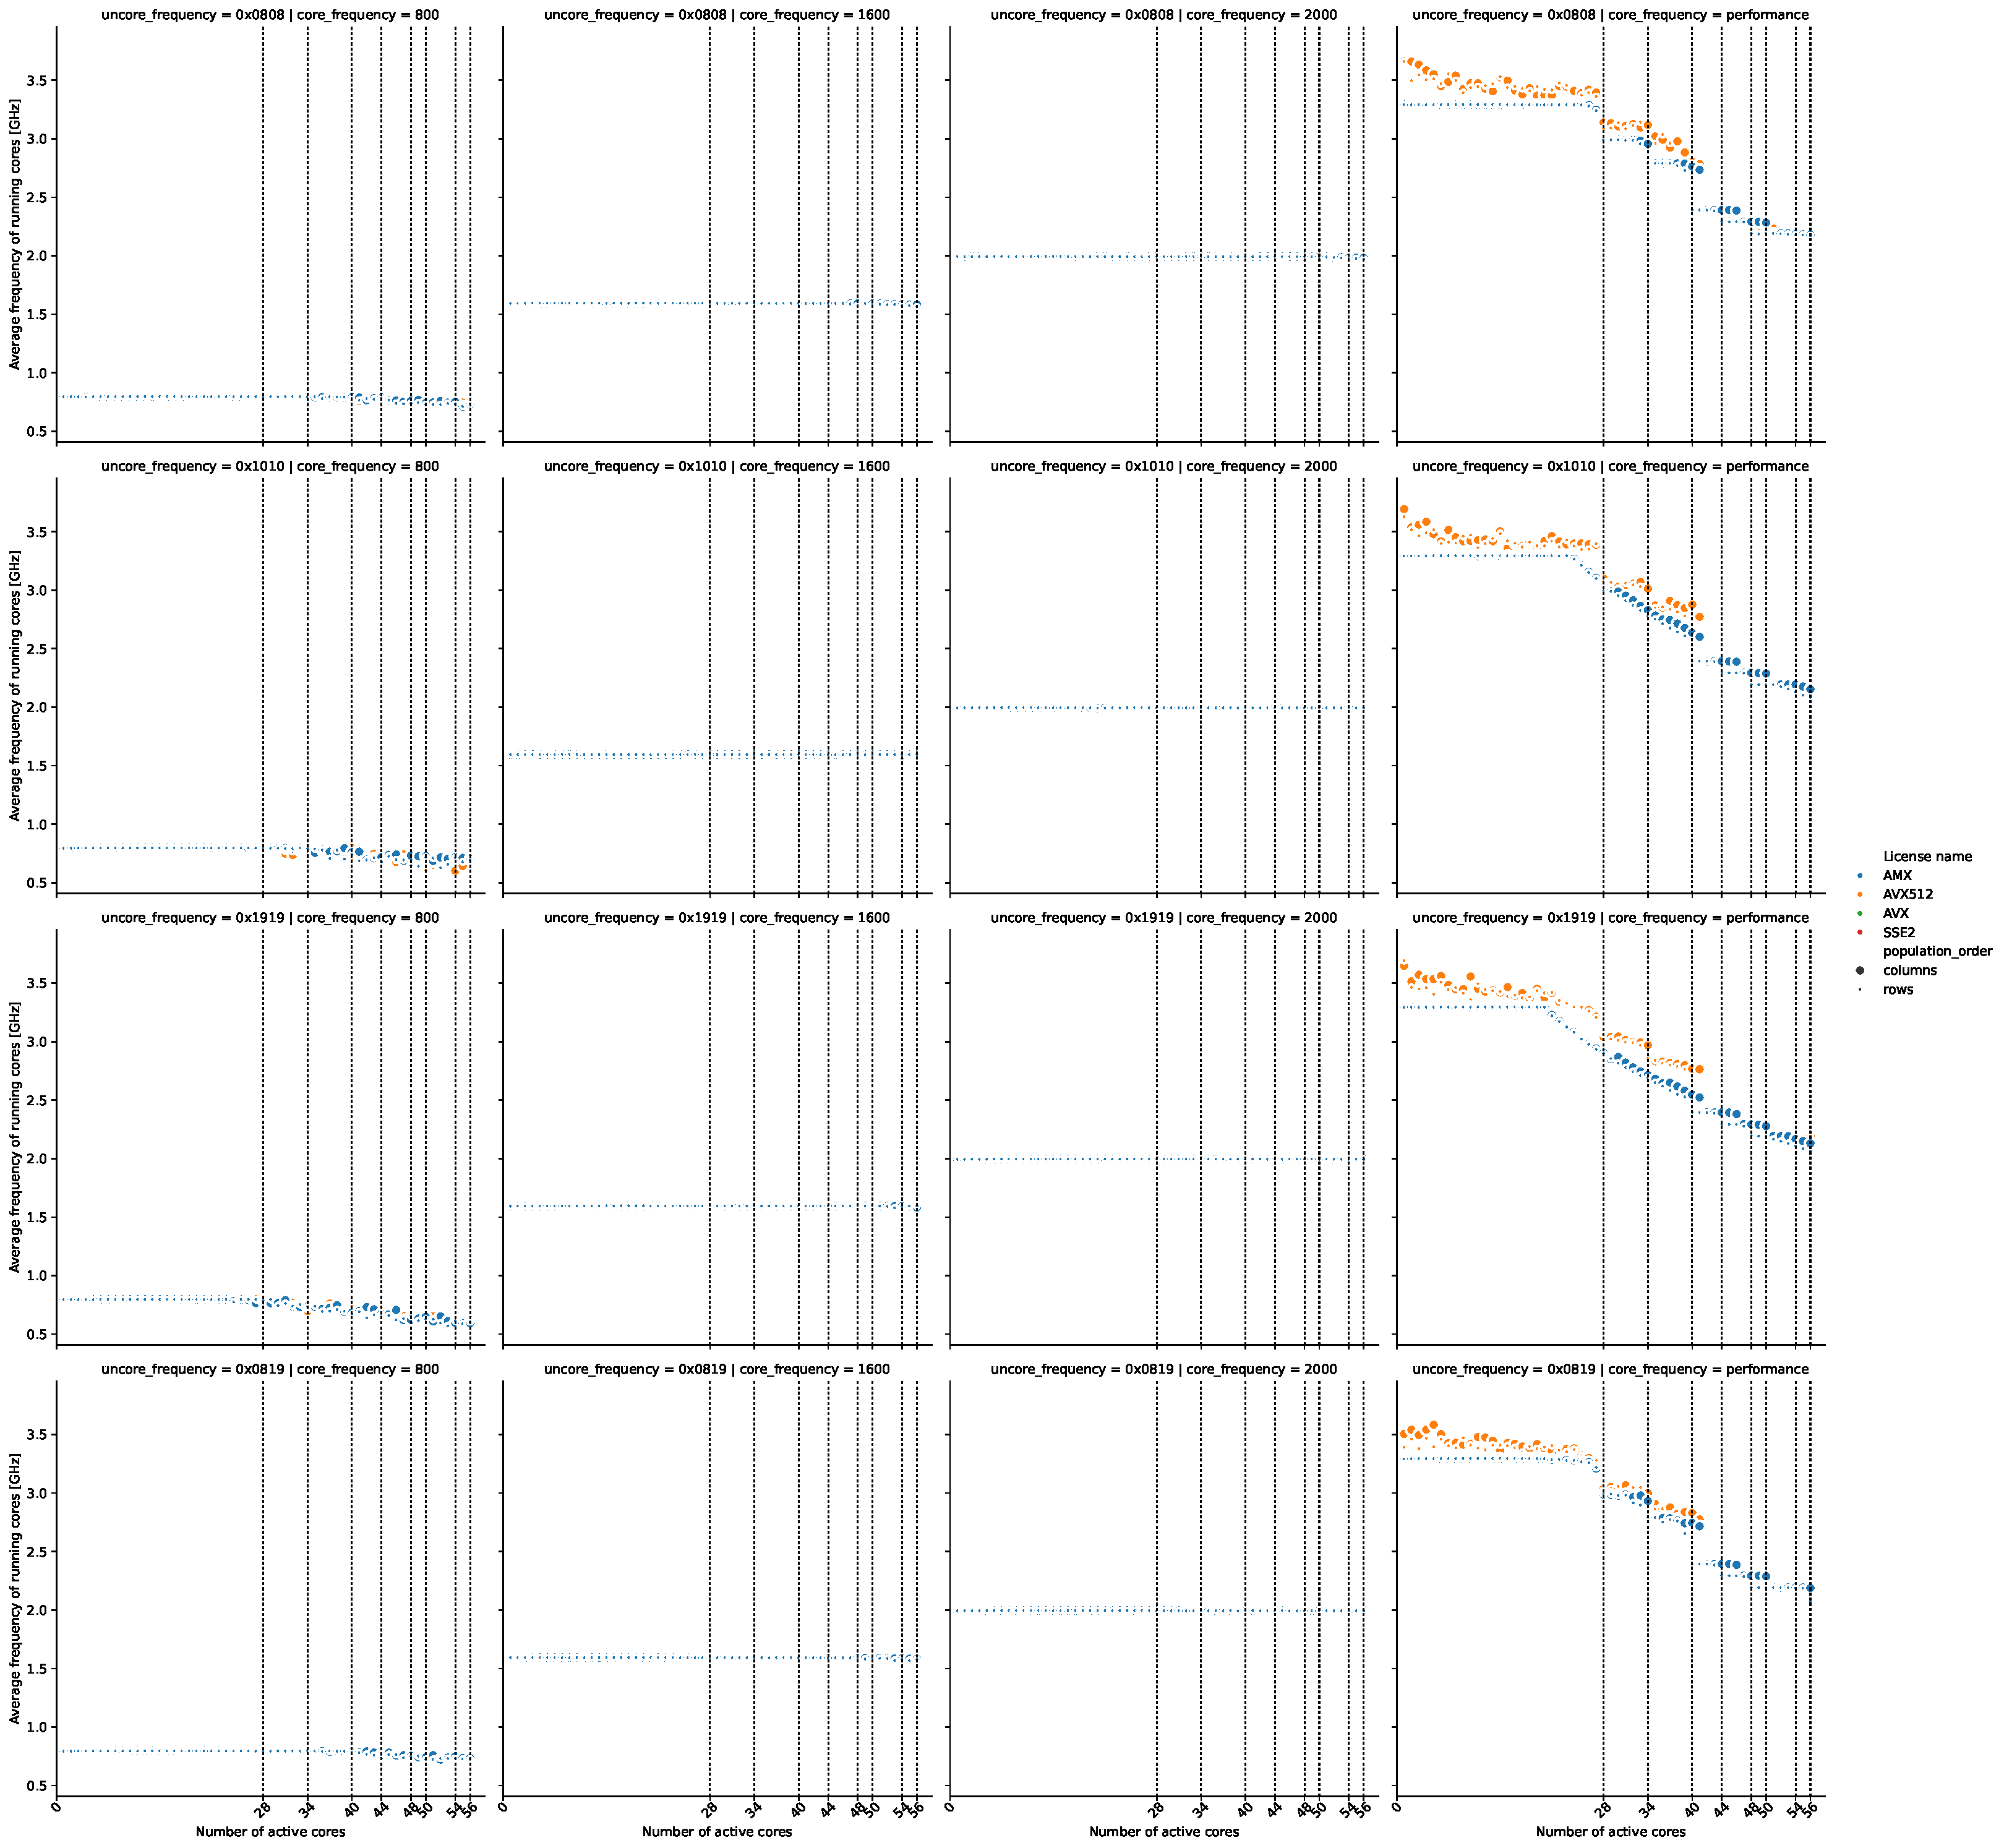
\includegraphics[width=\columnwidth]{fig/core-power-regulators-core-frequency.pdf}
    %\caption{\label{fig:validated-p0n-frequencies}Validation of the opportunistic AVX turbo frequencies of the test system extracted using Intel Speed Select Technology.
    %The number of active cores are split into eight buckets. The license and the bucket decides the resulting turbo frequency.
    %In the first bucket the SSE and AVX2 license bands share the same frequency. We make shure that the package power does not exceed the maximum of \SI{350}{\watt} of our test platfrom.}
\end{figure}

\begin{figure}[]
    \centering
    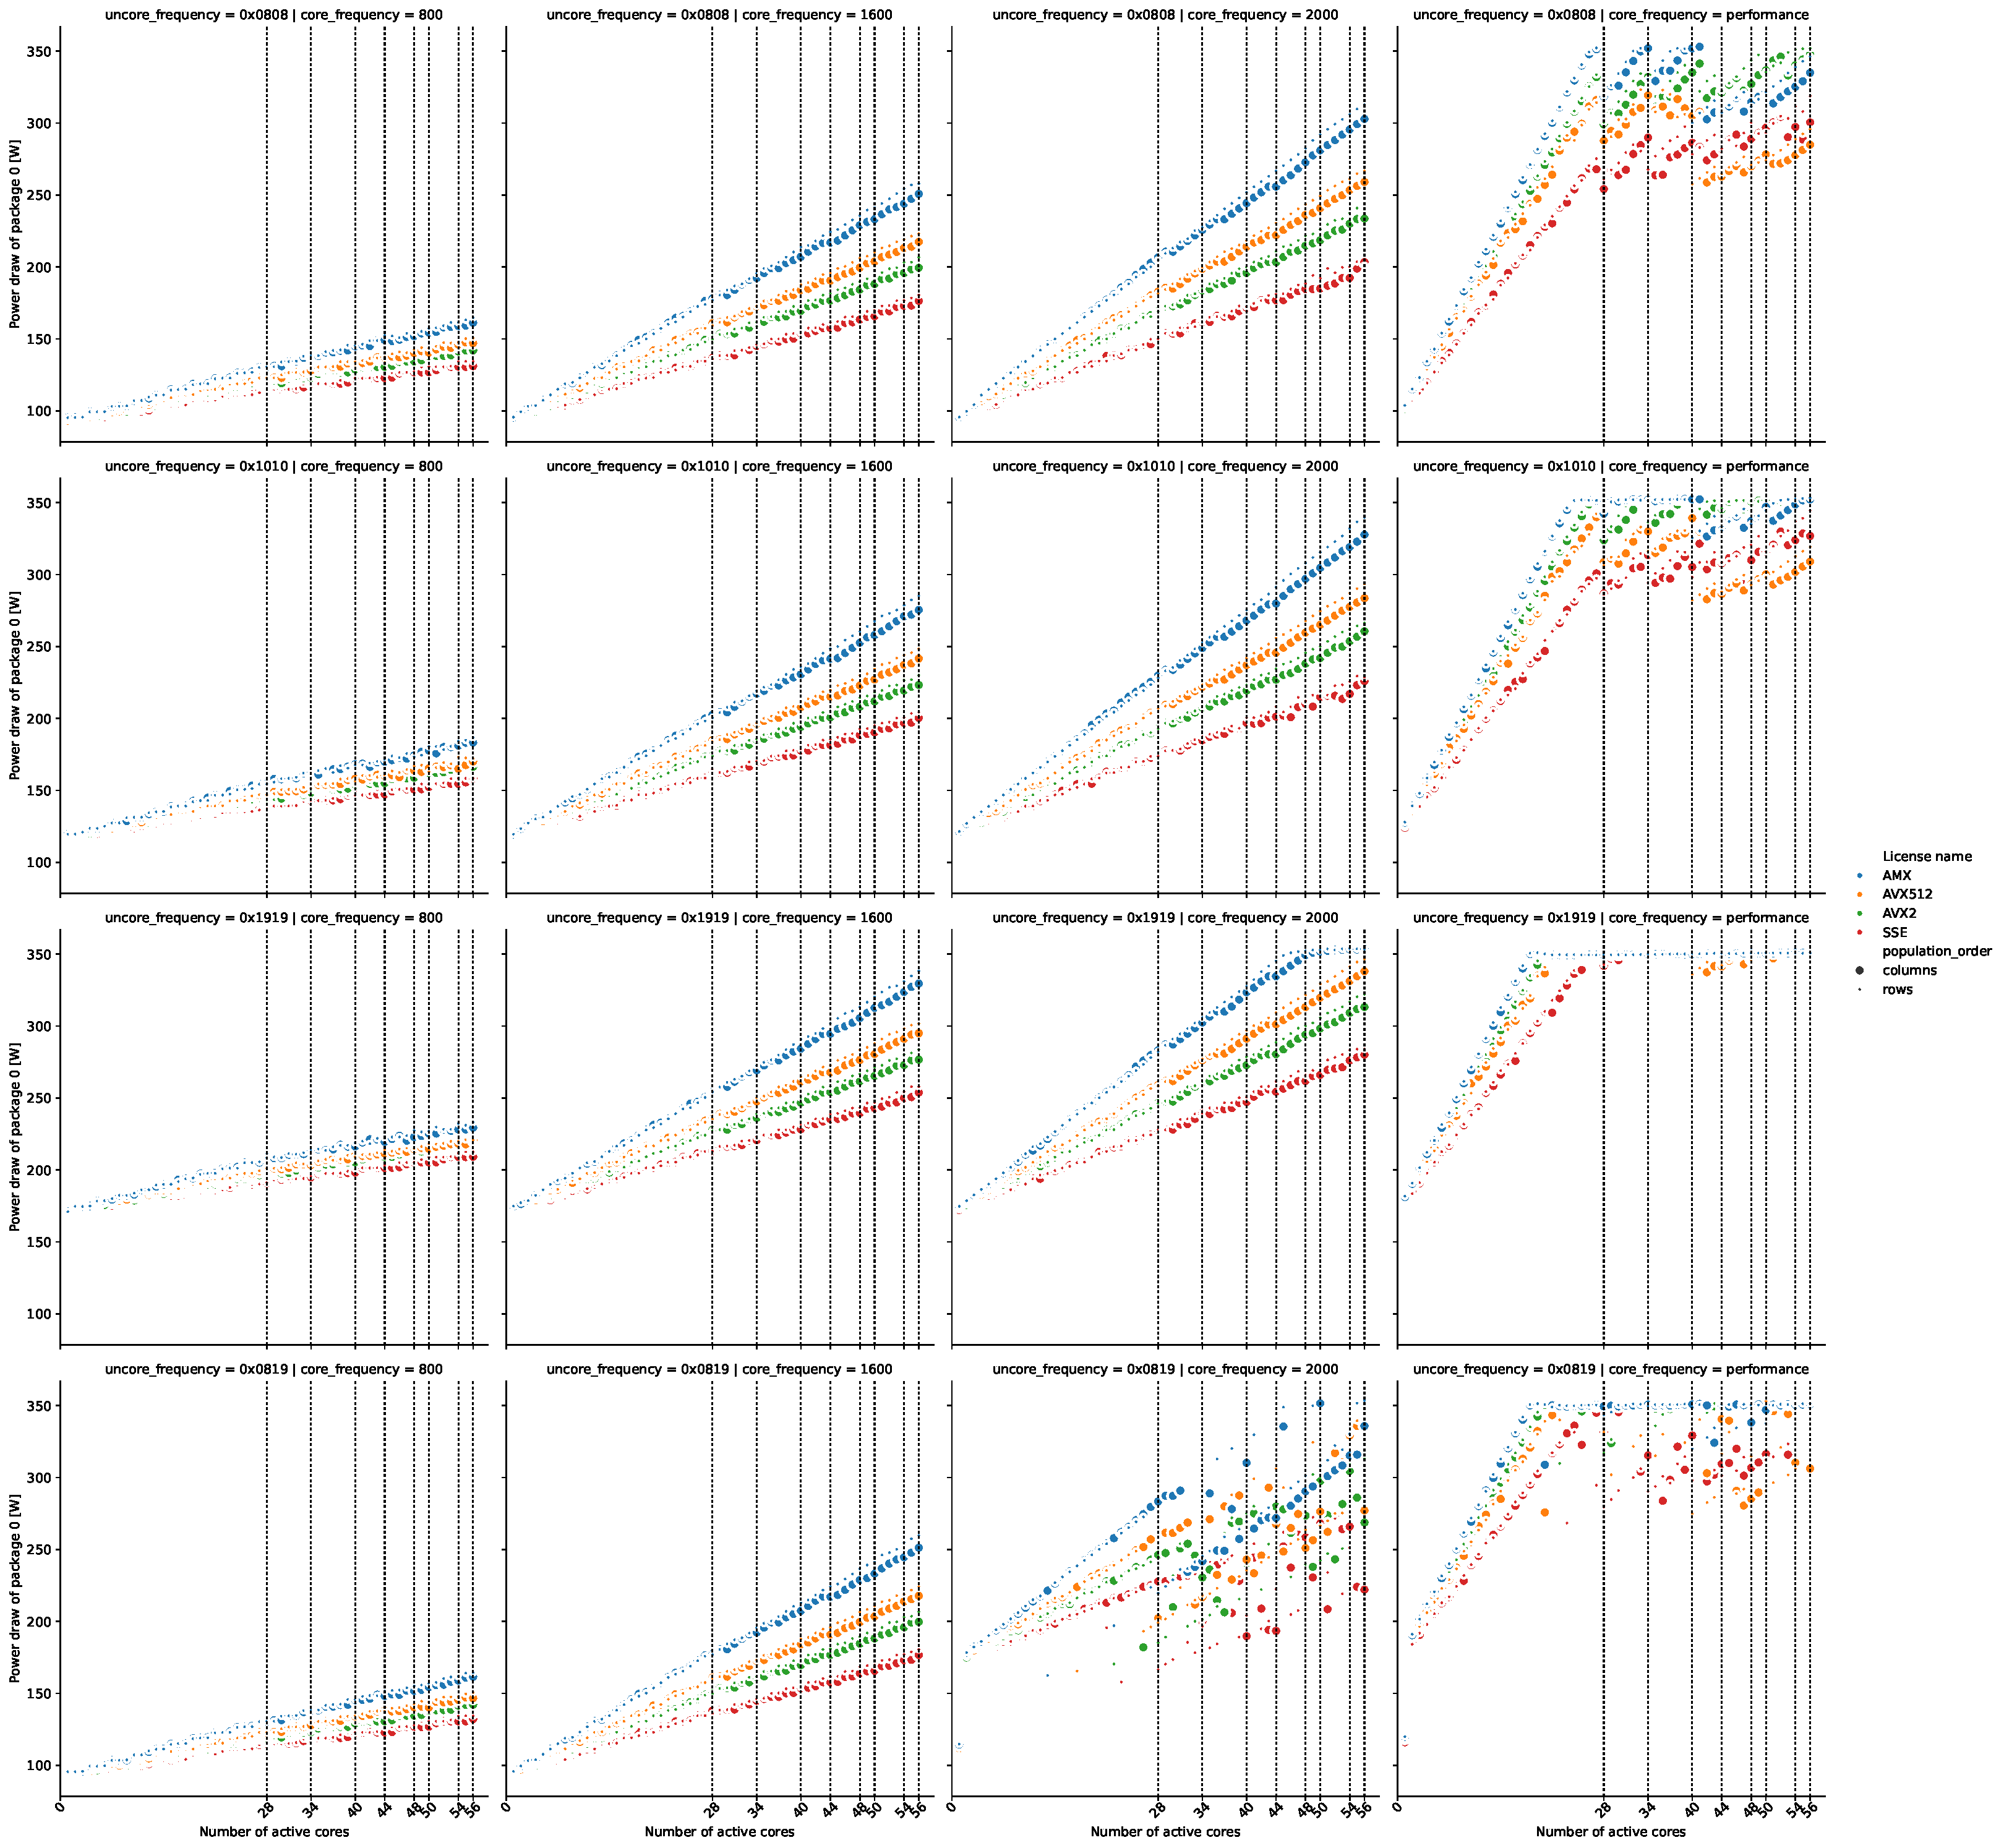
\includegraphics[width=\columnwidth]{fig/core-power-regulators-package-power.pdf}
    %\caption{\label{fig:validated-p0n-frequencies}Validation of the opportunistic AVX turbo frequencies of the test system extracted using Intel Speed Select Technology.
    %The number of active cores are split into eight buckets. The license and the bucket decides the resulting turbo frequency.
    %In the first bucket the SSE and AVX2 license bands share the same frequency. We make shure that the package power does not exceed the maximum of \SI{350}{\watt} of our test platfrom.}
\end{figure}


\section{Intel speed select}
\label{sec:isst}

\begin{itemize}
    \item intel speed select technology and avx frequencies are independent of one another.\\
    one plot to support this claim. potential for optimization on intels side.
    sort of: turbo-mode (turbo ratio limit) is one of many algorithm.
    turbo-freq buckets are another. (garanteed turbo freqs in high prio buckets, vs low prio)
    perf-profile is yet another. (different TRLs (?) and base frequencies with different number of cores)
    core-power with CLOS groups are another. (different frequency limits based on different priorities)
    base-freq
    \item open question: how do they work together?
\end{itemize}

\todoms{what does this do. what are the CLOS groups. cite the patent. how fast are the frequency transitions of the control loop?}


\section{P-State Latencies}

\todoms{Describe DVFS, latencies occur between switches, cite ftalat paper, schoene skylake and alderlake for comparison.}

To measure the latencies that occur during DVFS switches, I adapt ftalat, a benchmark developed by CITE PAPER, with modification by CITE PAPER.
ftalat measures the execution time of a compute loop with a fixed processor frequency.
The measurement methodology is as follows:
First, a frequency change is requested.
Second, the time until the execution time of the compute loop matches the expected for the requested frequency is measured.
Then the measurements waits a random time between \SI{0}{\us} and \SI{5000}{\us} before being repeated for \SI{1000}{} times.

In~\cite{Schoene_2024_Alder_Lake}, Schöne et al. demonstrated that the transition latencies for Alder Lake processors depend on the time since the last frequency transition.
In~\figref{pstate_latencies_time_dependance} we can observe this behaviour for frequency transitions from \SI{1.2}{\GHz} to \SI{1.9}{}, \SI{2.0}{} and \SI{2.1}{\GHz}, whilst the transition latency from \SI{1.2}{\GHz} to \SI{1.8}{\GHz} is unaffected by wait times.
We split the measurement data at a interval of \SI{1}{\ms} since the last frequency transition and plot the median latencies in~\figref{pstate_latencies_median}.
Below this interval the behaviour is the same as in Skylake-SP~\cite{Schoene_2019_SKL} with a higher latency of \SI{600}{\us} instead of \SI{500}{\us}.
Above this interval we see a different behaviour when switching to a higher frequency of \SI{1.9}{\GHz} and above.
Some source/target frequency pairs emit a higher transition latency, especially when switching to \SI{1.9}{\GHz} and \SI{2.0}{\GHz} from a lower frequency.
The expected worst case transition latency falls between \SI{1100}{\us} and \SI{2000}{\us}.
This can be read from the 99th percentile plot in~\figref{pstate_latencies_99percentQuantile}.
Outliers make this plot noiser than the other ones in this section.

\begin{figure}[]
    \begin{subfigure}[t]{0.45\linewidth}
        \centering
        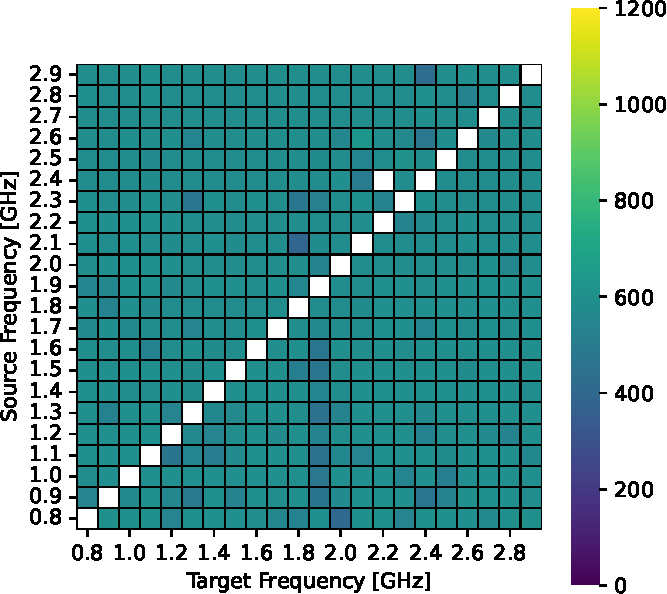
\includegraphics[width=\linewidth]{fig/ftalat_median_<1ms_hati.pdf}
        \caption{\label{fig:pstate_latencies_median_lt_1ms}Median p-state latencies. ($< \SI{1}{\ms}$)}
    \end{subfigure}
    \hfill
    \begin{subfigure}[t]{0.45\linewidth}
        \centering
        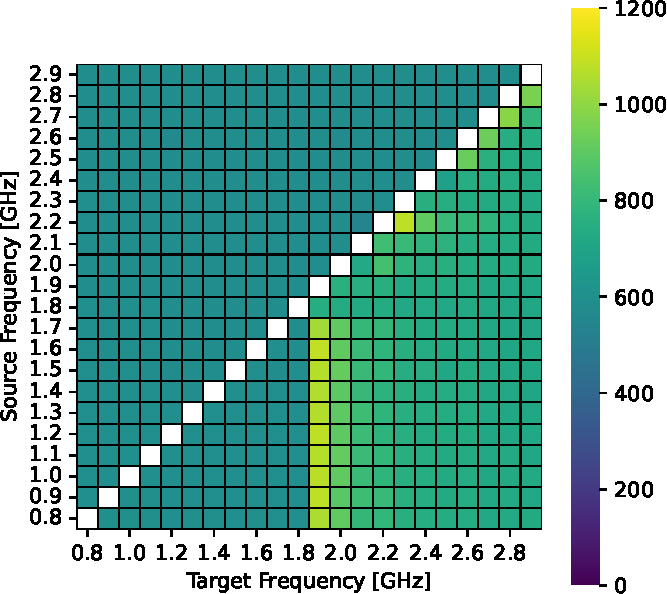
\includegraphics[width=\linewidth]{fig/ftalat_median_>1ms_hati.pdf}
        \caption{\label{fig:pstate_latencies_median_gt_1ms}Median p-state latencies. ($> \SI{1}{\ms}$)}
    \end{subfigure}
    \caption{\label{fig:pstate_latencies_median}Median P-State switching latencies of the Sapphire Rappids processor, differentiated by wait times between frequency transitions below and above \SI{1}{\ms}.}
\end{figure}

\begin{figure}[]
    \centering
    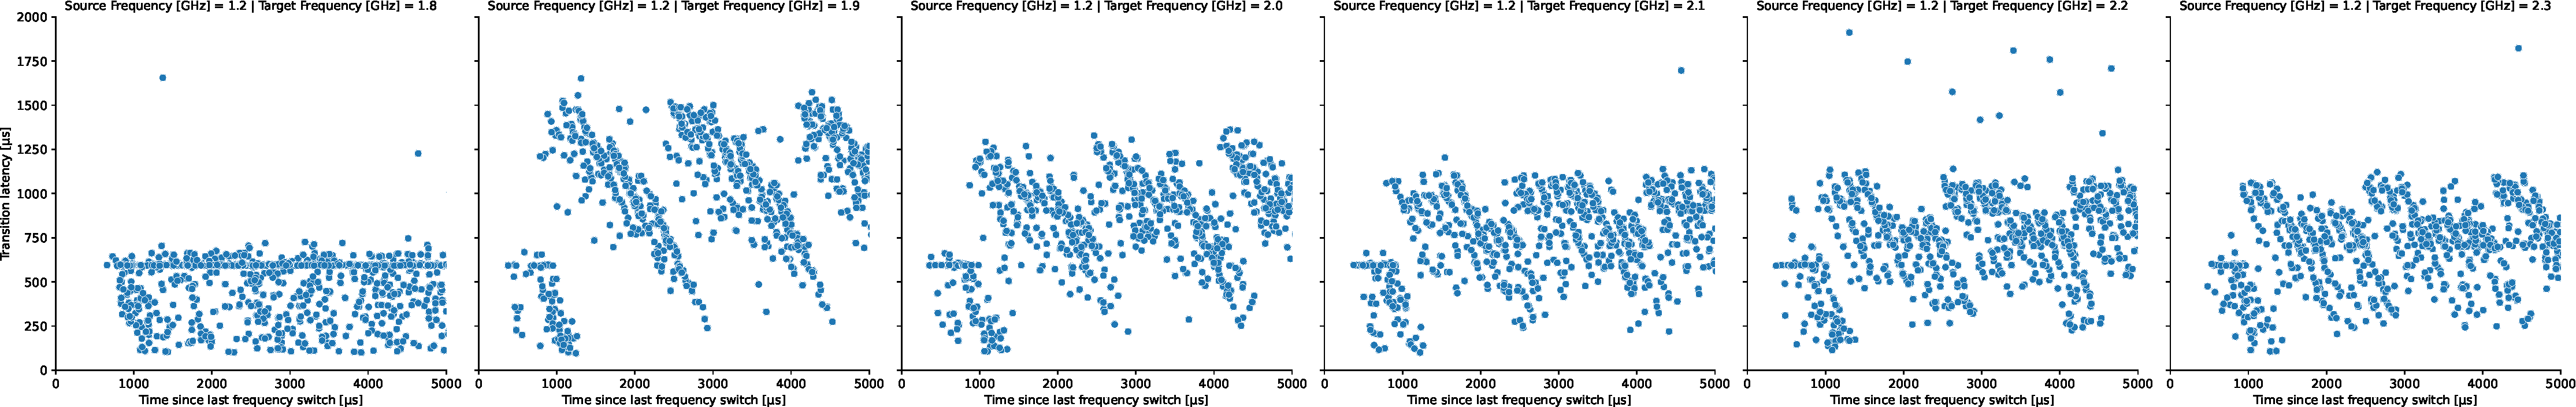
\includegraphics[width=\columnwidth]{fig/ftalat_scatter_wait_transition_latency_hati.pdf}
    \caption{\label{fig:pstate_latencies_time_dependance}Dependance of the time between frequency transitions on the transition latency. Displayed for frequency transitions from \SI{1.2}{\GHz} to \SI{1.8}{}, \SI{1.9}{}, \SI{2.0}{} and \SI{2.1}{\GHz}.}
\end{figure}

\begin{figure}[]
    \centering
    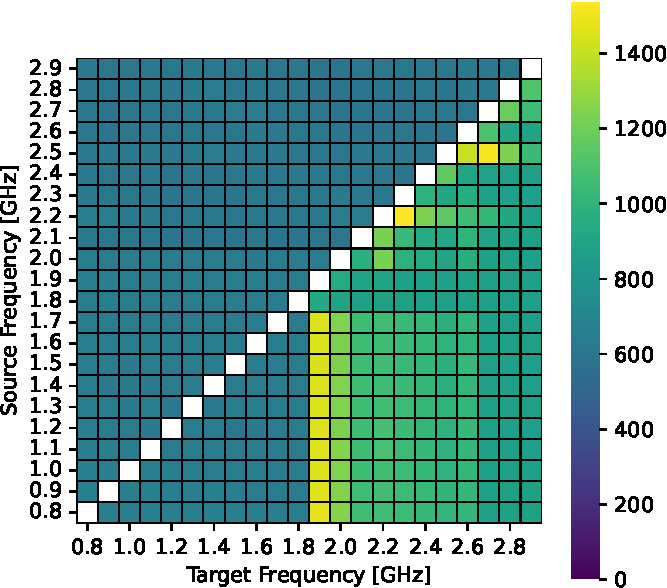
\includegraphics[width=0.45\columnwidth]{fig/ftalat_95percentQuantile_hati.pdf}
    \caption{\label{fig:pstate_latencies_95percentQuantile}95th percentile of P-state switching latencies.}
\end{figure}


\section{Uncore Frequency Scaling}
\todoms{timing of uncore frequency change. l1 ptr, swithing to l3 ptr chasing. scripts in skylake paper.}

\section{Idle State Latencies}
\todoms{Both user and normal C states latencies}
\todoms{influence of tiles on the c state latencies}
